\section{寄存器描述}
\regover{
{\hyperref[tmr-TCCR]{TCCR}}&Timer Clock Source
\\
\hline
{\hyperref[tmr-TMR2-0]{TMR2\_0}}&Timer2 Match Value 0
\\
\hline
{\hyperref[tmr-TMR2-1]{TMR2\_1}}&Timer2 Match Value 1
\\
\hline
{\hyperref[tmr-TMR2-2]{TMR2\_2}}&Timer2 Match Value 2
\\
\hline
{\hyperref[tmr-TMR3-0]{TMR3\_0}}&Timer3 Match Value 0
\\
\hline
{\hyperref[tmr-TMR3-1]{TMR3\_1}}&Timer3 Match Value 1
\\
\hline
{\hyperref[tmr-TMR3-2]{TMR3\_2}}&Timer3 Match Value 2
\\
\hline
{\hyperref[tmr-TCR2]{TCR2}}&Timer2 Counter Value
\\
\hline
{\hyperref[tmr-TCR3]{TCR3}}&Timer3 Counter Value
\\
\hline
{\hyperref[tmr-TSR2]{TSR2}}&Timer2 Match Status
\\
\hline
{\hyperref[tmr-TSR3]{TSR3}}&Timer3 Match Status
\\
\hline
{\hyperref[tmr-TIER2]{TIER2}}&Timer2 Match Interrupt Enable
\\
\hline
{\hyperref[tmr-TIER3]{TIER3}}&Timer3 Match Interrupt Enable
\\
\hline
{\hyperref[tmr-TPLVR2]{TPLVR2}}&Timer2 Pre-Load Value
\\
\hline
{\hyperref[tmr-TPLVR3]{TPLVR3}}&Timer3 Pre-Load Value
\\
\hline
{\hyperref[tmr-TPLCR2]{TPLCR2}}&Timer2 Pre-Load Control
\\
\hline
{\hyperref[tmr-TPLCR3]{TPLCR3}}&Timer3 Pre-Load Control
\\
\hline
{\hyperref[tmr-WMER]{WMER}}&Watch-dog reset/interrupt Mode
\\
\hline
{\hyperref[tmr-WMR]{WMR}}&Watch-dog Match Value
\\
\hline
{\hyperref[tmr-WVR]{WVR}}&Watch-dog Counter Value
\\
\hline
{\hyperref[tmr-WSR]{WSR}}&Watch-dog Reset Status
\\
\hline
{\hyperref[tmr-TICR2]{TICR2}}&Timer2 Interrupt Clear
\\
\hline
{\hyperref[tmr-TICR3]{TICR3}}&Timer3 Interrupt Clear
\\
\hline
{\hyperref[tmr-WICR]{WICR}}&WDT Interrupt Clear
\\
\hline
{\hyperref[tmr-TCER]{TCER}}&Timer Counter Enable/Clear
\\
\hline
{\hyperref[tmr-TCMR]{TCMR}}&Timer Counter Mode
\\
\hline
{\hyperref[tmr-TILR2]{TILR2}}&Timer2 Match Interrupt Mode
\\
\hline
{\hyperref[tmr-TILR3]{TILR3}}&Timer3 Match Interrupt Mode
\\
\hline
{\hyperref[tmr-WCR]{WCR}}&WDT Counter Reset
\\
\hline
{\hyperref[tmr-WFAR]{WFAR}}&WDT Access Key1
\\
\hline
{\hyperref[tmr-WSAR]{WSAR}}&WDT Access Key2
\\
\hline
{\hyperref[tmr-TCVWR2]{TCVWR2}}&Timer2 Counter Latch Value
\\
\hline
{\hyperref[tmr-TCVWR3]{TCVWR3}}&Timer3 Counter Latch Value
\\
\hline
{\hyperref[tmr-TCVSYN2]{TCVSYN2}}&Timer2 Counter Sync Value
\\
\hline
{\hyperref[tmr-TCVSYN3]{TCVSYN3}}&Timer3 Counter Sync Value
\\
\hline
{\hyperref[tmr-TCDR]{TCDR}}&Timer Division
\\
\hline
{\hyperref[tmr-GPIO]{GPIO}}&GPIO Mode
\\
\hline
{\hyperref[tmr-GPIO-LAT1]{GPIO\_LAT1}}&GPIO Latch Value1
\\
\hline
{\hyperref[tmr-GPIO-LAT2]{GPIO\_LAT2}}&GPIO Latch Value2
\\
\hline
{\hyperref[tmr-TCDR-FORCE]{TCDR\_FORCE}}&Timer Division Force
\\
\hline
}

\subsection{TCCR}
\label{tmr-TCCR}
地址:0x30009000
 \begin{figure}[H]
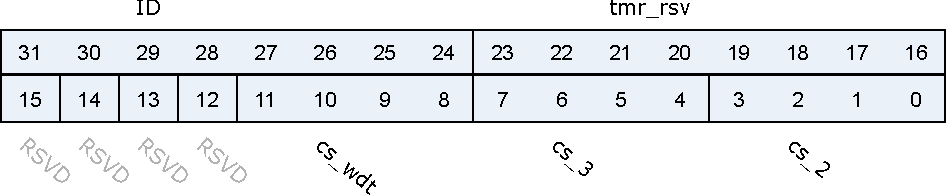
\includegraphics{tmr_TCCR.pdf}
\end{figure}

\regdes{31:24&ID&r&8'ha5&\\\hline
23:16&tmr\_rsv&rsvd&0&\\\hline
15:12&RSVD& & & \\\hline
11:8&cs\_wdt&r/w&4'd1&WDT  0:fclk  /  1:f32k  /  2:1k  /  3:32M  /  4:GPIO  /  5:No clock\\\hline
7:4&cs\_3&r/w&4'd5&Timer3  0:fclk  /  1:f32k  /  2:1k  /  3:32M  /  4:GPIO  /   5:No clock\\\hline
3:0&cs\_2&r/w&4'd5&Timer2  0:fclk  /  1:f32k  /  2:1k  /  3:32M  /  4:GPIO  /   5:No clock\\\hline

}
\subsection{TMR2\_0}
\label{tmr-TMR2-0}
地址:0x30009010
 \begin{figure}[H]
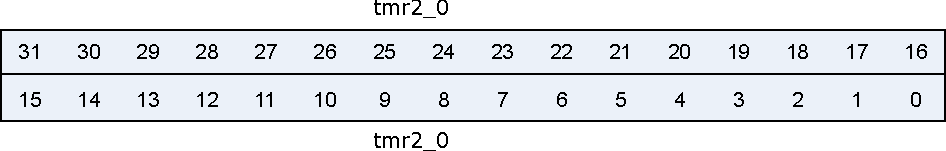
\includegraphics{tmr_TMR2_0.pdf}
\end{figure}

\regdes{31:0&tmr2\_0&r/w&32'hffffffff&Timer2 Match Value 0\\\hline

}
\subsection{TMR2\_1}
\label{tmr-TMR2-1}
地址:0x30009014
 \begin{figure}[H]
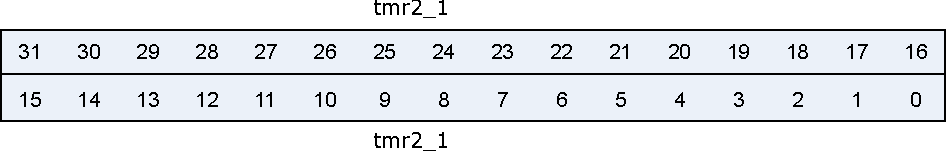
\includegraphics{tmr_TMR2_1.pdf}
\end{figure}

\regdes{31:0&tmr2\_1&r/w&32'hffffffff&Timer2 Match Value 1\\\hline

}
\subsection{TMR2\_2}
\label{tmr-TMR2-2}
地址:0x30009018
 \begin{figure}[H]
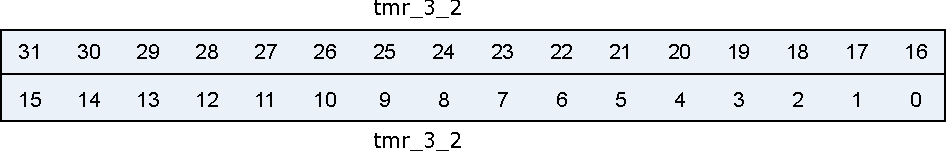
\includegraphics{tmr_TMR2_2.pdf}
\end{figure}

\regdes{31:0&tmr2\_2&r/w&32'hffffffff&Timer2 Match Value 2\\\hline

}
\subsection{TMR3\_0}
\label{tmr-TMR3-0}
地址:0x3000901c
 \begin{figure}[H]
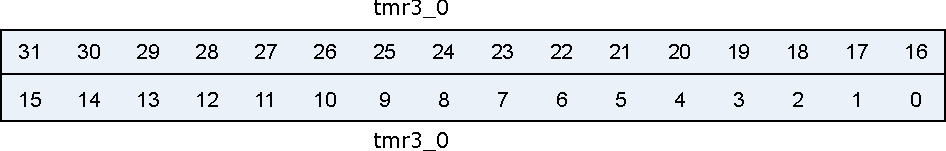
\includegraphics{tmr_TMR3_0.pdf}
\end{figure}

\regdes{31:0&tmr3\_0&r/w&32'hffffffff&Timer3 Match Value 0\\\hline

}
\subsection{TMR3\_1}
\label{tmr-TMR3-1}
地址:0x30009020
 \begin{figure}[H]
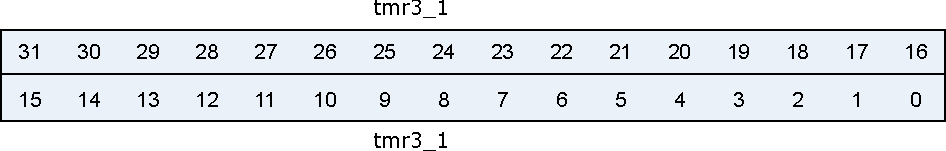
\includegraphics{tmr_TMR3_1.pdf}
\end{figure}

\regdes{31:0&tmr3\_1&r/w&32'hffffffff&Timer3 Match Value 1\\\hline

}
\subsection{TMR3\_2}
\label{tmr-TMR3-2}
地址:0x30009024
 \begin{figure}[H]
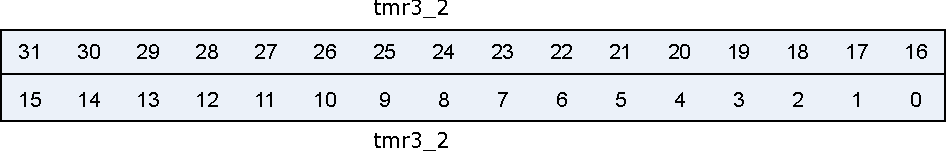
\includegraphics{tmr_TMR3_2.pdf}
\end{figure}

\regdes{31:0&tmr3\_2&r/w&32'hffffffff&Timer3 Match Value 2\\\hline

}
\subsection{TCR2}
\label{tmr-TCR2}
地址:0x3000902c
 \begin{figure}[H]
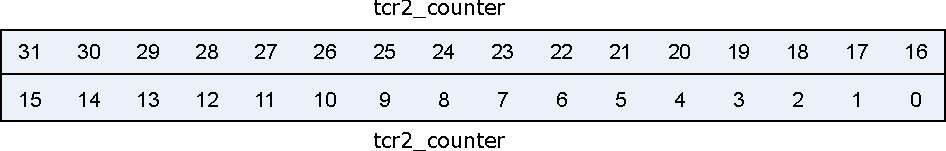
\includegraphics{tmr_TCR2.pdf}
\end{figure}

\regdes{31:0&tcr2\_cnt&r&0&Timer2 Counter Value\\\hline

}
\subsection{TCR3}
\label{tmr-TCR3}
地址:0x30009030
 \begin{figure}[H]
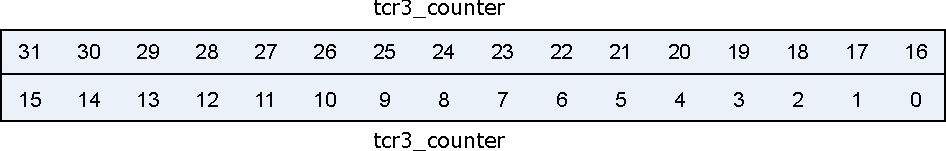
\includegraphics{tmr_TCR3.pdf}
\end{figure}

\regdes{31:0&tcr3\_cnt&r&0&Timer3 Counter Value\\\hline

}
\subsection{TSR2}
\label{tmr-TSR2}
地址:0x30009038
 \begin{figure}[H]
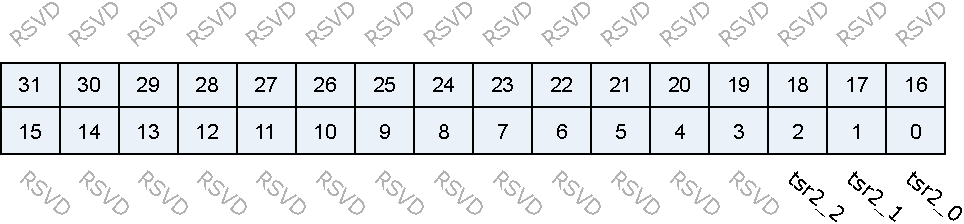
\includegraphics{tmr_TSR2.pdf}
\end{figure}

\regdes{31:3&RSVD& & & \\\hline
2&tsr2\_2&r&0&Timer2 match value 2 status/Clear interrupt would also clear this bit\\\hline
1&tsr2\_1&r&0&Timer2 match value 1 status/Clear interrupt would also clear this bit\\\hline
0&tsr2\_0&r&0&Timer2 match value 0 status/Clear interrupt would also clear this bit\\\hline

}
\subsection{TSR3}
\label{tmr-TSR3}
地址:0x3000903c
 \begin{figure}[H]
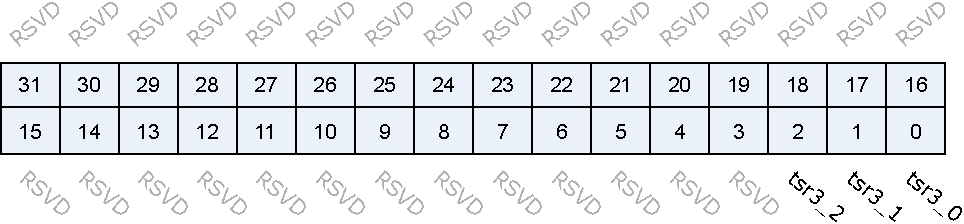
\includegraphics{tmr_TSR3.pdf}
\end{figure}

\regdes{31:3&RSVD& & & \\\hline
2&tsr3\_2&r&0&Timer3 match value 2 status/Clear interrupt would also clear this bit\\\hline
1&tsr3\_1&r&0&Timer3 match value 1 status/Clear interrupt would also clear this bit\\\hline
0&tsr3\_0&r&0&Timer3 match value 0 status/Clear interrupt would also clear this bit\\\hline

}
\subsection{TIER2}
\label{tmr-TIER2}
地址:0x30009044
 \begin{figure}[H]
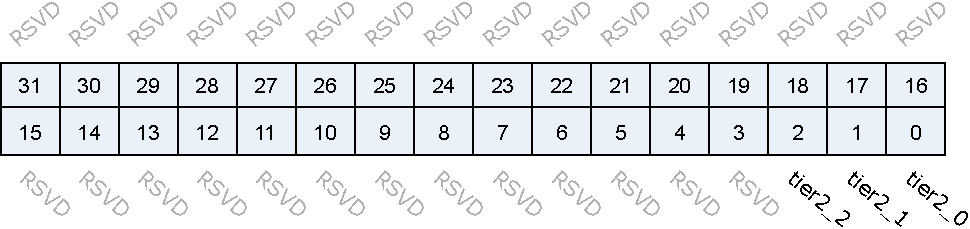
\includegraphics{tmr_TIER2.pdf}
\end{figure}

\regdes{31:3&RSVD& & & \\\hline
2&tier2\_2&r/w&0&Timer2 match value 2 interrupt enable\\\hline
1&tier2\_1&r/w&0&Timer2 match value 1 interrupt enable\\\hline
0&tier2\_0&r/w&0&Timer2 match value 0 interrupt enable\\\hline

}
\subsection{TIER3}
\label{tmr-TIER3}
地址:0x30009048
 \begin{figure}[H]
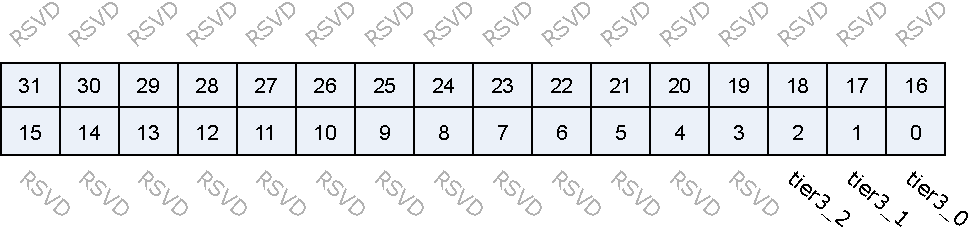
\includegraphics{tmr_TIER3.pdf}
\end{figure}

\regdes{31:3&RSVD& & & \\\hline
2&tier3\_2&r/w&0&Timer3 match value 2 interrupt enable\\\hline
1&tier3\_1&r/w&0&Timer3 match value 1 interrupt enable\\\hline
0&tier3\_0&r/w&0&Timer3 match value 0 interrupt enable\\\hline

}
\subsection{TPLVR2}
\label{tmr-TPLVR2}
地址:0x30009050
 \begin{figure}[H]
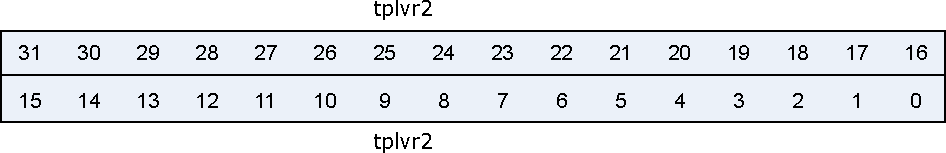
\includegraphics{tmr_TPLVR2.pdf}
\end{figure}

\regdes{31:0&tplvr2&r/w&0&Timer2 Pre-Load Value\\\hline

}
\subsection{TPLVR3}
\label{tmr-TPLVR3}
地址:0x30009054
 \begin{figure}[H]
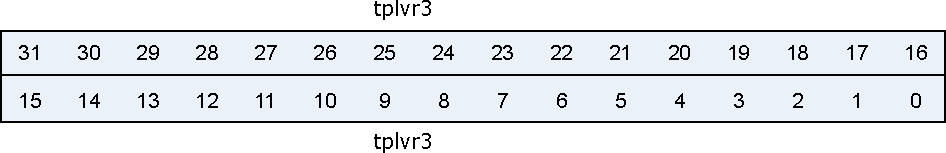
\includegraphics{tmr_TPLVR3.pdf}
\end{figure}

\regdes{31:0&tplvr3&r/w&0&Timer3 Pre-Load Value\\\hline

}
\subsection{TPLCR2}
\label{tmr-TPLCR2}
地址:0x3000905c
 \begin{figure}[H]
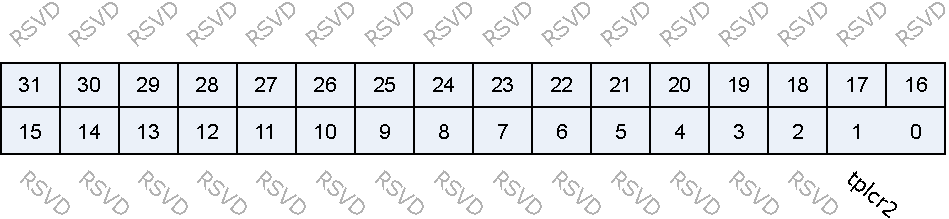
\includegraphics{tmr_TPLCR2.pdf}
\end{figure}

\regdes{31:2&RSVD& & & \\\hline
1:0&tplcr2&r/w&0&Timer2 pre-load control \par 2'd0 - No pre-load \par 2'd1 - Pre-load with match comparator 0 \par 2'd2 - Pre-load with match comparator 1 \par 2'd3 - Pre-load with match comparator 2
\\\hline

}
\subsection{TPLCR3}
\label{tmr-TPLCR3}
地址:0x30009060
 \begin{figure}[H]
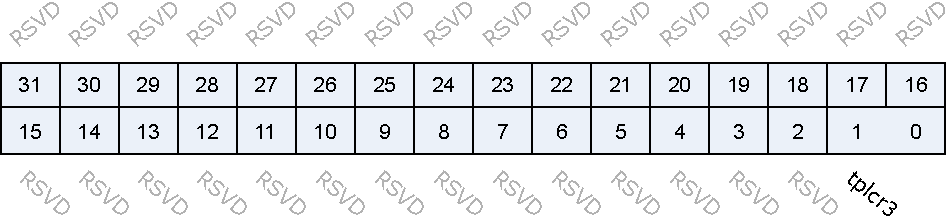
\includegraphics{tmr_TPLCR3.pdf}
\end{figure}

\regdes{31:2&RSVD& & & \\\hline
1:0&tplcr3&r/w&0&Timer3 pre-load control \par 2'd0 - No pre-load \par 2'd1 - Pre-load with match comparator 0 \par 2'd2 - Pre-load with match comparator 1 \par 2'd3 - Pre-load with match comparator 2
\\\hline

}
\subsection{WMER}
\label{tmr-WMER}
地址:0x30009064
 \begin{figure}[H]
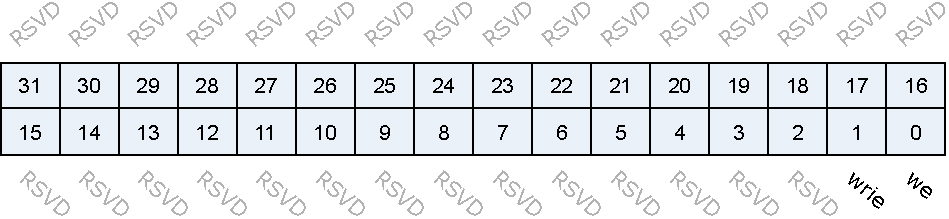
\includegraphics{tmr_WMER.pdf}
\end{figure}

\regdes{31:2&RSVD& & & \\\hline
1&wrie&r/w&0&WDT reset/interrupt mode \par 1'b0 - WDT expiration to generate interrupt \par 1'b1 - WDT expiration to generate reset source
\\\hline
0&we&r/w&0&WDT enable register\\\hline

}
\subsection{WMR}
\label{tmr-WMR}
地址:0x30009068
 \begin{figure}[H]
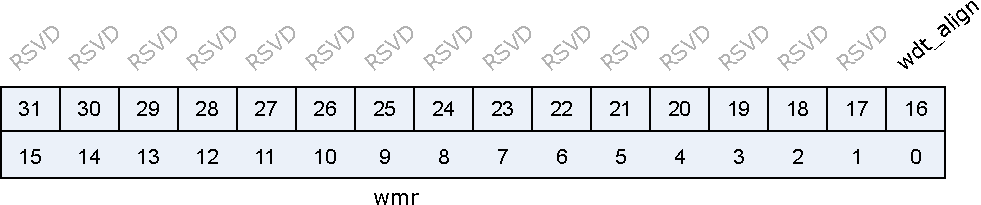
\includegraphics{tmr_WMR.pdf}
\end{figure}

\regdes{31:17&RSVD& & & \\\hline
16&wdt\_align&r/w&0&WDT compare value update align interrupt\\\hline
15:0&wmr&r/w&16'hffff&WDT counter match value\\\hline

}
\subsection{WVR}
\label{tmr-WVR}
地址:0x3000906c
 \begin{figure}[H]
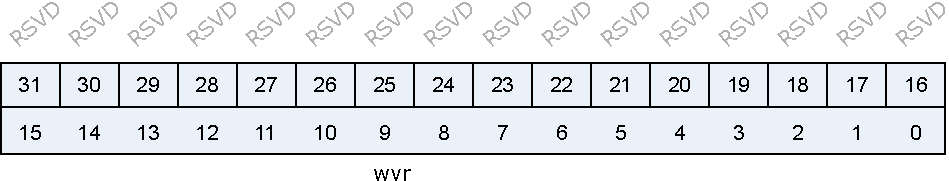
\includegraphics{tmr_WVR.pdf}
\end{figure}

\regdes{31:16&RSVD& & & \\\hline
15:0&wdt\_cnt&r&0&WDT counter value\\\hline

}
\subsection{WSR}
\label{tmr-WSR}
地址:0x30009070
 \begin{figure}[H]
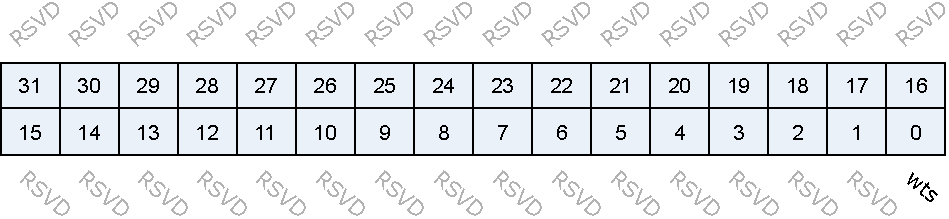
\includegraphics{tmr_WSR.pdf}
\end{figure}

\regdes{31:1&RSVD& & & \\\hline
0&wts&w&0&WDT reset status \par Write 0 to clear the WDT reset status \par Read 1 indicates reset was caused by the WDT
\\\hline

}
\subsection{TICR2}
\label{tmr-TICR2}
地址:0x30009078
 \begin{figure}[H]
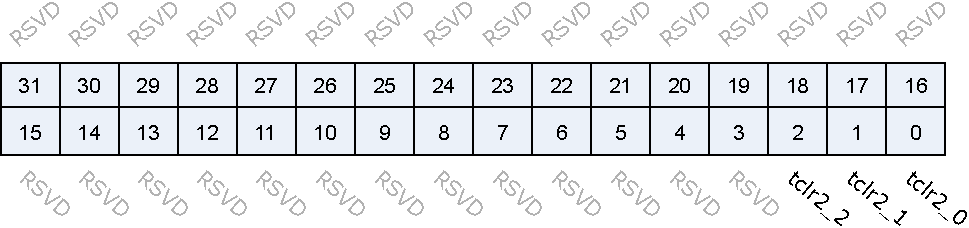
\includegraphics{tmr_TICR2.pdf}
\end{figure}

\regdes{31:3&RSVD& & & \\\hline
2&tclr2\_2&w&0&Timer2 Interrupt clear for match comparator 2\\\hline
1&tclr2\_1&w&0&Timer2 Interrupt clear for match comparator 1\\\hline
0&tclr2\_0&w&0&Timer2 Interrupt clear for match comparator 0\\\hline

}
\subsection{TICR3}
\label{tmr-TICR3}
地址:0x3000907c
 \begin{figure}[H]
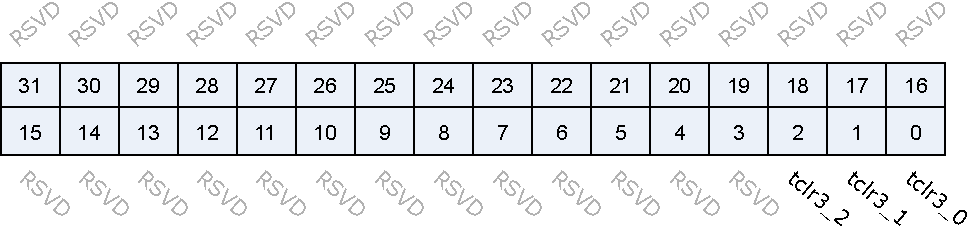
\includegraphics{tmr_TICR3.pdf}
\end{figure}

\regdes{31:3&RSVD& & & \\\hline
2&tclr3\_2&w&0&Timer3 Interrupt clear for match comparator 2\\\hline
1&tclr3\_1&w&0&Timer3 Interrupt clear for match comparator 1\\\hline
0&tclr3\_0&w&0&Timer3 Interrupt clear for match comparator 0\\\hline

}
\subsection{WICR}
\label{tmr-WICR}
地址:0x30009080
 \begin{figure}[H]
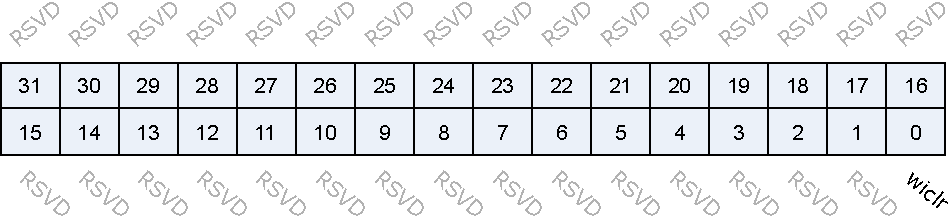
\includegraphics{tmr_WICR.pdf}
\end{figure}

\regdes{31:1&RSVD& & & \\\hline
0&wiclr&w&0&WDT Interrupt Clear\\\hline

}
\subsection{TCER}
\label{tmr-TCER}
地址:0x30009084
 \begin{figure}[H]
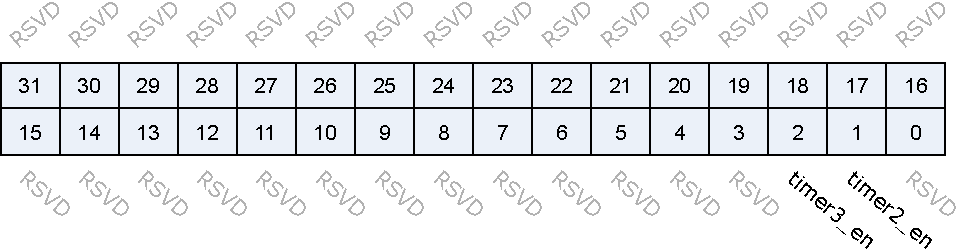
\includegraphics{tmr_TCER.pdf}
\end{figure}

\regdes{31:7&RSVD& & & \\\hline
6&tcr3\_cnt\_clr&r/w&0&Timer3 count clear\\\hline
5&tcr2\_cnt\_clr&r/w&0&Timer2 count clear\\\hline
4:3&RSVD& & & \\\hline
2&timer3\_en&r/w&0&Timer3 count enable\\\hline
1&timer2\_en&r/w&0&Timer2 count enable\\\hline
0&RSVD& & & \\\hline

}
\subsection{TCMR}
\label{tmr-TCMR}
地址:0x30009088
 \begin{figure}[H]
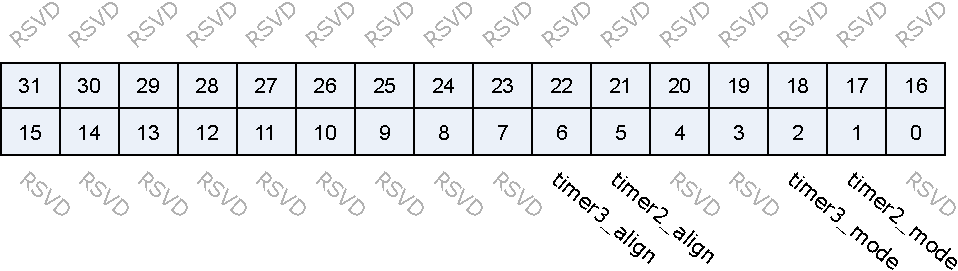
\includegraphics{tmr_TCMR.pdf}
\end{figure}

\regdes{31:7&RSVD& & & \\\hline
6&timer3\_align&r/w&0&Timer3 compare value update align interrupt\\\hline
5&timer2\_align&r/w&0&Timer2 compare value update align interrupt\\\hline
4:3&RSVD& & & \\\hline
2&timer3\_mode&r/w&0&0:pre-load mode  1:free run mode\\\hline
1&timer2\_mode&r/w&0&0:pre-load mode  1:free run mode\\\hline
0&RSVD& & & \\\hline

}
\subsection{TILR2}
\label{tmr-TILR2}
地址:0x30009090
 \begin{figure}[H]
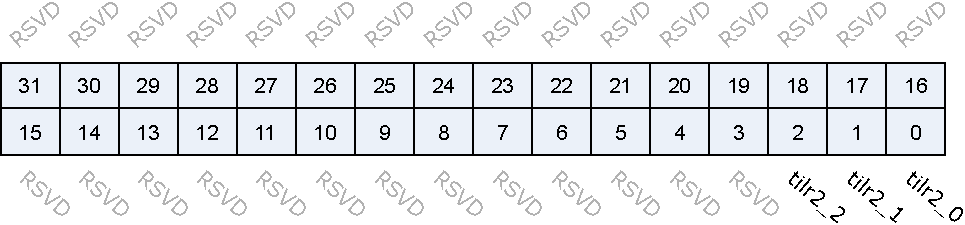
\includegraphics{tmr_TILR2.pdf}
\end{figure}

\regdes{31:3&RSVD& & & \\\hline
2&tilr2\_2&r/w&0&0:level   1:edge\\\hline
1&tilr2\_1&r/w&0&0:level   1:edge\\\hline
0&tilr2\_0&r/w&0&0:level   1:edge\\\hline

}
\subsection{TILR3}
\label{tmr-TILR3}
地址:0x30009094
 \begin{figure}[H]
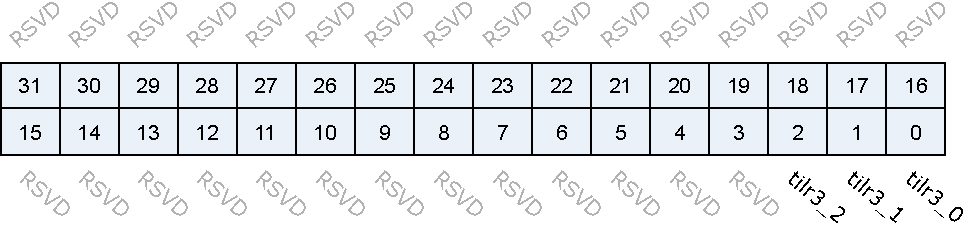
\includegraphics{tmr_TILR3.pdf}
\end{figure}

\regdes{31:3&RSVD& & & \\\hline
2&tilr3\_2&r/w&0&0:level   1:edge\\\hline
1&tilr3\_1&r/w&0&0:level   1:edge\\\hline
0&tilr3\_0&r/w&0&0:level   1:edge\\\hline

}
\subsection{WCR}
\label{tmr-WCR}
地址:0x30009098
 \begin{figure}[H]
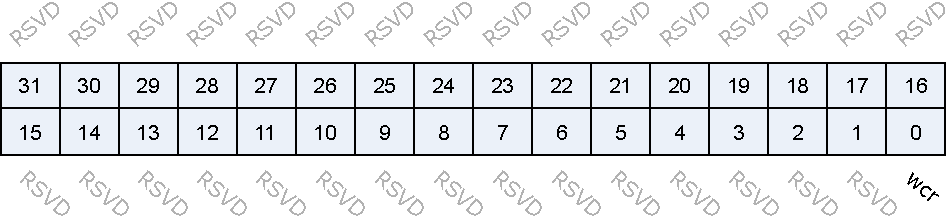
\includegraphics{tmr_WCR.pdf}
\end{figure}

\regdes{31:1&RSVD& & & \\\hline
0&wcr&w&0&WDT Counter Reset\\\hline

}
\subsection{WFAR}
\label{tmr-WFAR}
地址:0x3000909c
 \begin{figure}[H]
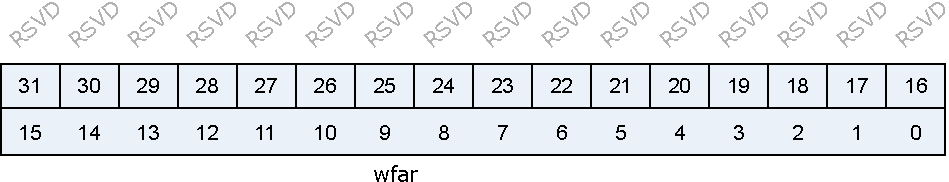
\includegraphics{tmr_WFAR.pdf}
\end{figure}

\regdes{31:16&RSVD& & & \\\hline
15:0&wfar&w&0&WDT access key1 - 16'hBABA\\\hline

}
\subsection{WSAR}
\label{tmr-WSAR}
地址:0x300090a0
 \begin{figure}[H]
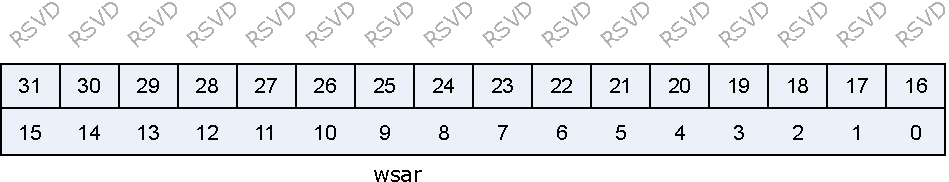
\includegraphics{tmr_WSAR.pdf}
\end{figure}

\regdes{31:16&RSVD& & & \\\hline
15:0&wsar&w&0&WDT access key2 - 16'hEB10\\\hline

}
\subsection{TCVWR2}
\label{tmr-TCVWR2}
地址:0x300090a8
 \begin{figure}[H]
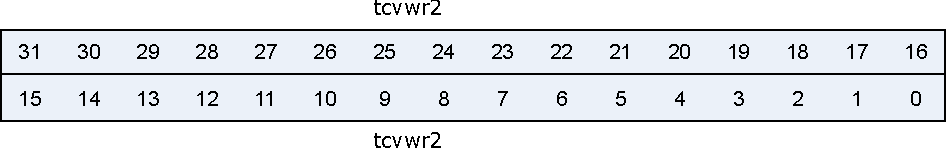
\includegraphics{tmr_TCVWR2.pdf}
\end{figure}

\regdes{31:0&tcr2\_cnt\_lat&r&0&Timer2 Counter Latch Value\\\hline

}
\subsection{TCVWR3}
\label{tmr-TCVWR3}
地址:0x300090ac
 \begin{figure}[H]
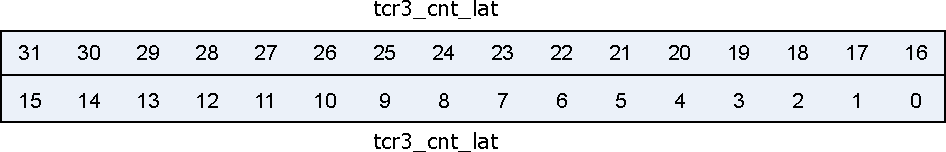
\includegraphics{tmr_TCVWR3.pdf}
\end{figure}

\regdes{31:0&tcr3\_cnt\_lat&r&0&Timer3 Counter Latch Value\\\hline

}
\subsection{TCVSYN2}
\label{tmr-TCVSYN2}
地址:0x300090b4
 \begin{figure}[H]
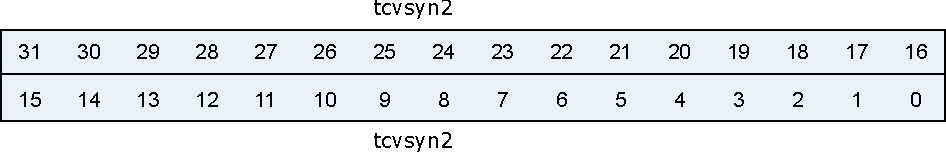
\includegraphics{tmr_TCVSYN2.pdf}
\end{figure}

\regdes{31:0&tcr2\_cnt\_sync&r&0&Timer2 Counter Sync Value (continue readable)\\\hline

}
\subsection{TCVSYN3}
\label{tmr-TCVSYN3}
地址:0x300090b8
 \begin{figure}[H]
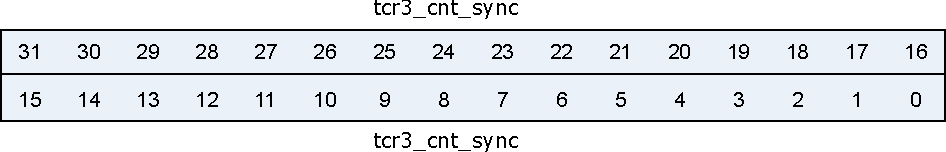
\includegraphics{tmr_TCVSYN3.pdf}
\end{figure}

\regdes{31:0&tcr3\_cnt\_sync&r&0&Timer3 Counter Sync Value (continue readable)\\\hline

}
\subsection{TCDR}
\label{tmr-TCDR}
地址:0x300090bc
 \begin{figure}[H]
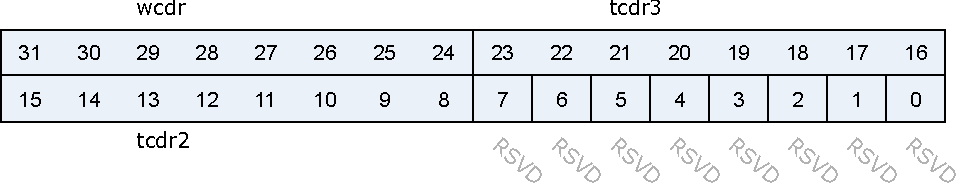
\includegraphics{tmr_TCDR.pdf}
\end{figure}

\regdes{31:24&wcdr&r/w&0&WDT clock division value register\\\hline
23:16&tcdr3&r/w&0&Timer3 clock division value register\\\hline
15:8&tcdr2&r/w&0&Timer2 clock division value register\\\hline
7:0&RSVD& & & \\\hline

}
\subsection{GPIO}
\label{tmr-GPIO}
地址:0x300090c0
 \begin{figure}[H]
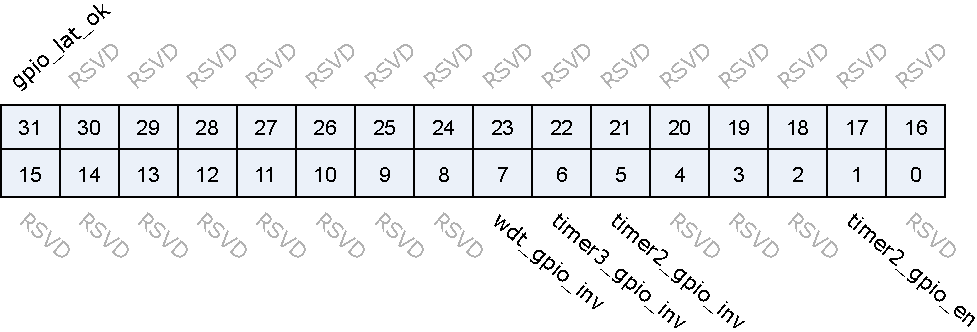
\includegraphics{tmr_GPIO.pdf}
\end{figure}

\regdes{31&gpio\_lat\_ok&r&0&Latch Done. Pulse width = (GPIO\_LAT2 - GPIO\_LAT1) * (Timer2 Cycle)\\\hline
30:8&RSVD& & & \\\hline
7&wdt\_gpio\_inv&r/w&0&WDT gpio polarity  0:pos  1:neg\\\hline
6&timer3\_gpio\_inv&r/w&0&Timer3 gpio polarity  0:pos  1:neg\\\hline
5&timer2\_gpio\_inv&r/w&0&Timer2 gpio polarity  0:pos  1:neg\\\hline
4:2&RSVD& & & \\\hline
1&timer2\_gpio\_en&r/w&0&Timer2 gpio measure enable\\\hline
0&RSVD& & & \\\hline

}
\subsection{GPIO\_LAT1}
\label{tmr-GPIO-LAT1}
地址:0x300090c4
 \begin{figure}[H]
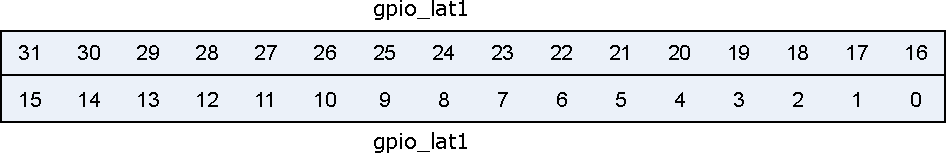
\includegraphics{tmr_GPIO_LAT1.pdf}
\end{figure}

\regdes{31:0&gpio\_lat1&r&0&Pos-Edge Latch Timer2\\\hline

}
\subsection{GPIO\_LAT2}
\label{tmr-GPIO-LAT2}
地址:0x300090c8
 \begin{figure}[H]
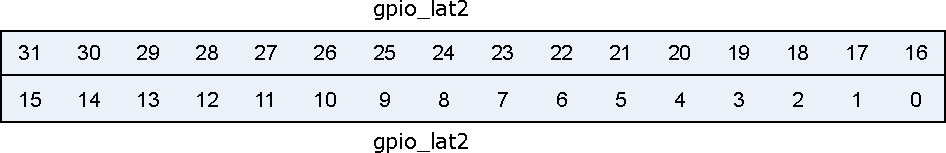
\includegraphics{tmr_GPIO_LAT2.pdf}
\end{figure}

\regdes{31:0&gpio\_lat2&r&0&Neg-Edge Latch Timer2\\\hline

}
\subsection{TCDR\_FORCE}
\label{tmr-TCDR-FORCE}
地址:0x300090cc
 \begin{figure}[H]
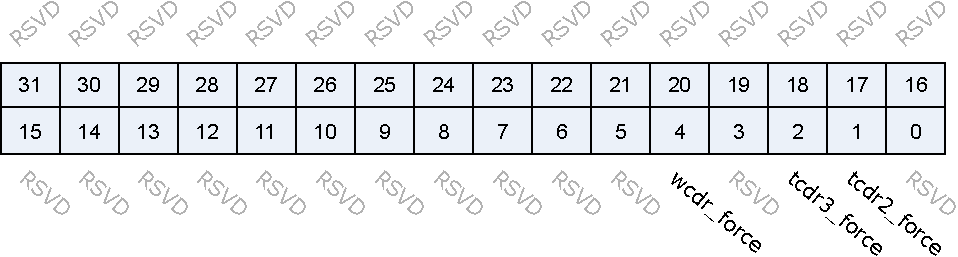
\includegraphics{tmr_TCDR_FORCE.pdf}
\end{figure}

\regdes{31:5&RSVD& & & \\\hline
4&wcdr\_force&r/w&0&Force WDT clock division value to counter\\\hline
3&RSVD& & & \\\hline
2&tcdr3\_force&r/w&0&Force Timer3 clock division value to counter\\\hline
1&tcdr2\_force&r/w&0&Force Timer2 clock division value to counter\\\hline
0&RSVD& & & \\\hline

}
